\begin{figure}
	\centering
	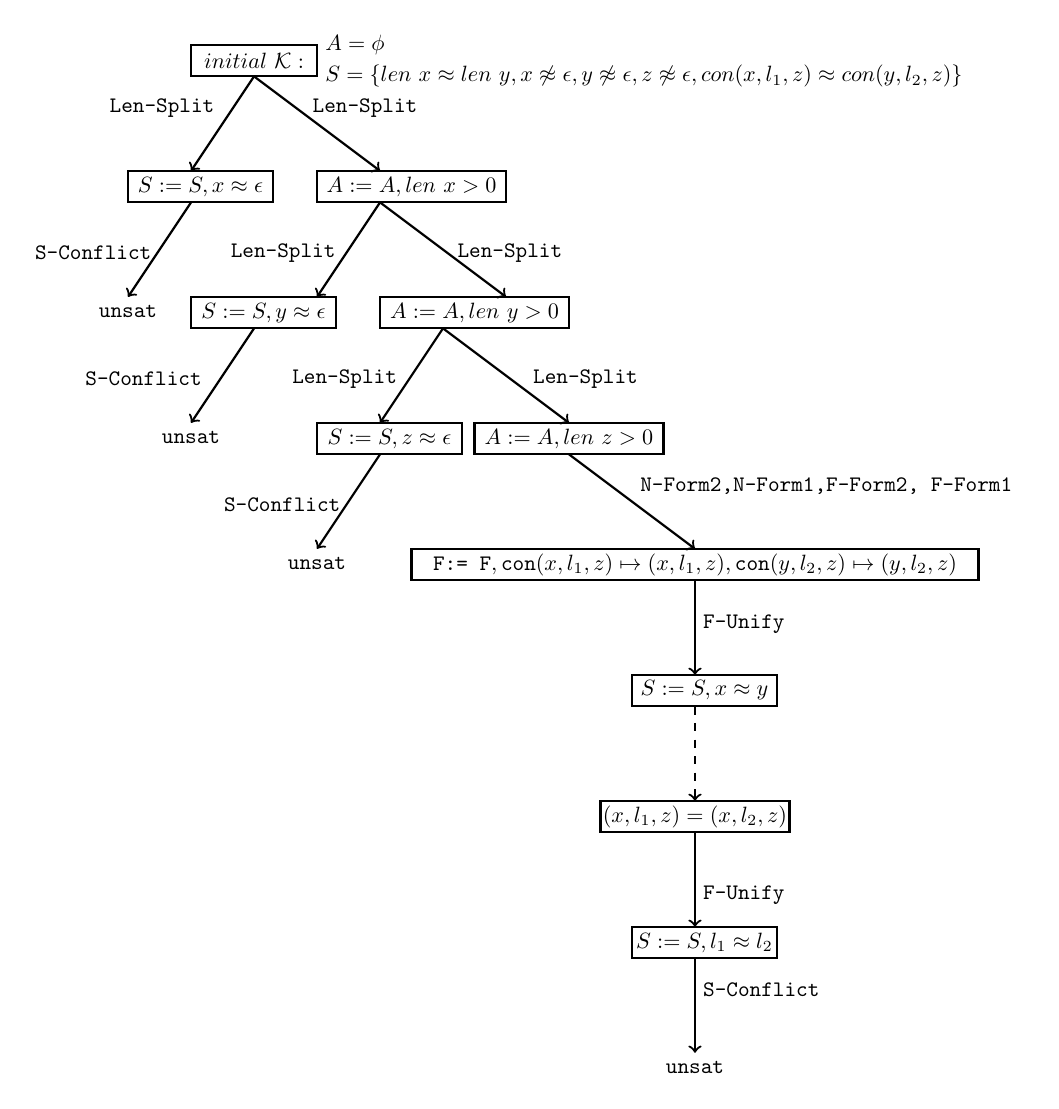
\begin{tikzpicture}[thick,scale=0.8, every node/.style={transform shape}]
	
	\node [right] at (3,20) { $ A=\phi $};
	\node [right] at (3,19.5) { $ S=\{  len \ x \approx len \ y, x \not\approx \epsilon, y \not\approx \epsilon,
		z \not\approx \epsilon, con (x, l_1,z) \approx con (y, l_2, z)\} $}; 
	 
    \draw (1,20) rectangle (3,19.5) node[pos=.5] {$ initial \ \mathcal{K}:$};
	
	\draw [->] (2,19.5) -- (1,18);
	\node [left] at (1.5,19) {$\texttt{Len-Split}$};
	
	\draw [->] (2,19.5) -- (4,18);
	\node [right] at (2.8,19) {$\texttt{Len-Split}$};
	
	
	\draw (0,18) rectangle (2.3,17.5) node[pos=.5] {$S:=S, x\approx \epsilon$};
	\node [rectangle, below] at (1,18) {};
	
	
	\draw (3,18) rectangle (6,17.5) node[pos=.5] {$A:=A, len \ x  > 0$};
	\node [rectangle, below] at (4,18) {};
	
	\draw [->] (1,17.5) -- (0,16);
	\node [left] at (0.5,16.7) {$\texttt{S-Conflict}$};
	
	\draw [->] (4,17.5) -- (3,16);
	\node [right] at (1.5,16.7) {$\texttt{Len-Split}$};
	\draw [->] (4,17.5) -- (6,16);
	\node [right] at (5.1,16.7) {$\texttt{Len-Split}$};
	
	\node [below] at (0,16) {$\texttt{unsat}$};
	\draw (1,16) rectangle (3.3,15.5) node[pos=.5] {$S:=S, y\approx \epsilon$};
	\node [below] at (2,16) {};
	\draw (4,16) rectangle (7,15.5) node[pos=.5] {$A:=A, len \ y  > 0$};
	\node [below] at (5,16) {};
	
	\draw [->] (2,15.5) -- (1,14);
	\node [left] at (1.3,14.7) {$\texttt{S-Conflict}$};
	\draw [->] (5,15.5) -- (4,14);
	\node [left] at (4.4,14.7) {$\texttt{Len-Split}$};	
	\draw [->] (5,15.5) -- (7,14);
	\node [right] at (6.3,14.7) {$\texttt{Len-Split}$};
	
	
	\node [below] at (1,14) {$\texttt{unsat}$};
	\draw (3,14) rectangle (5.3,13.5) node[pos=.5] {$S:=S, z\approx \epsilon$};
	\node [below] at (4,14) {};
	\draw (5.5,14) rectangle (8.5,13.5) node[pos=.5] {$A:=A, len \ z  > 0$};
	\node [below] at (7,14) {};


	\draw [->] (4,13.5) -- (3,12);
	\node [left] at (3.5,12.7) {$\texttt{S-Conflict}$};
	\draw [->] (7,13.5) -- (9,12);
    \node [right] at (8,13) {$\texttt{N-Form2,N-Form1,F-Form2, F-Form1 }$};
    

	
	\node [below] at (3,12) {$\texttt{unsat}$};
	\draw (4.5,12) rectangle (13.5,11.5) node[pos=.5] {$\texttt{F:= F},\texttt{con}(x,l_1,z)\mapsto (x,l_1,z),\texttt{con}(y,l_2,z)\mapsto(y,l_2,z)$};
	\node [below] at (9,12) {};
	
	\draw [->] (9,11.5) -- (9,10);
	\node [right] at (9,10.8) {$\texttt{F-Unify}$};
	
	\draw (8,10) rectangle (10.3,9.5) node[pos=.5] {$S:=S, x\approx y$};
	\node [below] at (9,10) {};
	
	\draw [dashed,->] (9,9.5) -- (9,8);
	
	\draw (7.5,8) rectangle (10.5,7.5) node[pos=.5] {$( x, l_1, z ) = (x, l_2,z)$};
	\node [below] at (9,8) {};
	
	\draw [->] (9,7.5) -- (9,6);
	\node [right] at (9,6.5) {$\texttt{F-Unify}$};
	
	\draw (8,6) rectangle (10.3,5.5) node[pos=.5] {$S:=S, l_1 \approx l_2$};
	\node [below] at (9,6) {};
	
	\draw [->] (9,5.5) -- (9,4);
	\node [right] at (9,5) {$\texttt{S-Conflict}$};
	
	\node [below] at (9,4) {$\texttt{unsat}$};
	
	
	
	
	
	
	\end{tikzpicture}
	\caption{The derivation tree for example 1. Here $l_1, l_2 $ are distinct constants of same length.}
\end{figure}	
